%=======================================================================
%  Satellite embeddings, text and night lights for municipal GDP -- final presentation
%  Plan and storyline: PRESENTATION_PLAN.md. Same design as the mid-term deck (presentation/midterm), whose
%  assets it reuses; new figures come from reports/figures and assets/ (make_figures.py or make_maps_local.py,
%  website screenshots). Footer route line: Problem, Approach, Test, Results, Failures, Application, Wrap-up.
%  Build (XeLaTeX, Lato; uses the system font or MiKTeX's Lato files):
%     cd presentation/final && latexmk -xelatex slides.tex
%=======================================================================
\documentclass[aspectratio=169,10pt]{beamer}
\usefonttheme{professionalfonts}
\usepackage{fontspec}
\IfFontExistsTF{Lato}{%
  \setsansfont{Lato}\newfontfamily\blackfont{Lato Black}\newfontfamily\lightfont{Lato Light}}{%
  \setsansfont{Lato-Regular.ttf}[BoldFont=Lato-Bold.ttf,ItalicFont=Lato-Italic.ttf,BoldItalicFont=Lato-BoldItalic.ttf]
  \newfontfamily\blackfont{Lato-Black.ttf}\newfontfamily\lightfont{Lato-Light.ttf}}
\usepackage{amsmath,amssymb}
\usepackage{booktabs,array,graphicx,xcolor}
\usepackage[normalem]{ulem}
\usepackage{tikz}
\usetikzlibrary{arrows.meta,positioning,calc,fit,backgrounds}
\graphicspath{{assets/}{../midterm/assets/}{../../reports/figures/}}

%------------------------- palette (same hex as make_figures.py) --------
\definecolor{night}{HTML}{0B1328}
\definecolor{night2}{HTML}{16223F}
\definecolor{glow}{HTML}{F2B134}
\definecolor{paper}{HTML}{F7F5F0}
\definecolor{ink}{HTML}{1E2433}
\definecolor{muted}{HTML}{687082}
\definecolor{rule}{HTML}{D9D5CC}
\definecolor{cimg}{HTML}{138A8A}
\definecolor{ctxt}{HTML}{7057C9}
\definecolor{cntl}{HTML}{E19A1F}
\definecolor{cgdp}{HTML}{C4493B}
\definecolor{cpoi}{HTML}{4A6FA5}
\definecolor{okc}{HTML}{2E8B57}
\definecolor{haze}{HTML}{AEB8D0}

%------------------------- beamer basics --------------------------------
\setbeamertemplate{navigation symbols}{}
\setbeamersize{text margin left=0.6cm,text margin right=0.6cm}
\setbeamercolor{normal text}{fg=ink}
\setbeamercolor{structure}{fg=ink}
\setbeamercolor{alerted text}{fg=cgdp}
\setbeamerfont{frametitle}{size=\fontsize{15}{18},series=\bfseries}
\setbeamertemplate{itemize item}{\raisebox{0.25ex}{\color{muted}\rule{0.4em}{0.4em}}}
\setbeamertemplate{enumerate item}{\color{cntl}\bfseries\insertenumlabel}
\setbeamertemplate{footline}{\vskip0.78cm}   % room for the footer drawn in the background
\setbeamertemplate{frametitle}{%
  \vskip0.36cm%
  \begin{beamercolorbox}[wd=\paperwidth,leftskip=0.6cm,rightskip=0.6cm]{frametitle}%
    \usebeamerfont{frametitle}\color{ink}\insertframetitle\par\vskip4pt%
    {\color{glow}\rule{1.1cm}{2.2pt}}%
  \end{beamercolorbox}\vskip0.02cm}
\hyphenpenalty=10000 \exhyphenpenalty=10000

%------------------------- route line in the footer ---------------------
\gdef\curstage{0}
\newcommand{\setstage}[1]{\gdef\curstage{#1}}
\newcommand{\paperbg}{%
  
\begin{tikzpicture}
    \useasboundingbox (0,0) rectangle (\paperwidth,\paperheight);
    \fill[paper] (0,0) rectangle (\paperwidth,\paperheight);
    \draw[rule,line width=0.4pt] (0.6cm,0.62cm) -- (\paperwidth-0.6cm,0.62cm);
    \node[anchor=west,font=\fontsize{6.5}{8}\selectfont,text=muted,inner sep=0] at (0.6cm,0.36cm)
      {Group 2 \ $\cdot$ \ GIS term project \ $\cdot$ \ final presentation};
    \node[anchor=east,font=\bfseries\fontsize{7}{8}\selectfont,text=ink,inner sep=0] at (\paperwidth-0.6cm,0.36cm)
      {\insertframenumber\,/\,\inserttotalframenumber};
    \ifnum\curstage>0
      \draw[rule,line width=1.2pt] (\paperwidth-9.2cm,0.36cm) -- (\paperwidth-1.7cm,0.36cm);
      \ifnum\curstage>1 \draw[ink,line width=1.2pt] (\paperwidth-9.2cm,0.36cm) -- ++({(\curstage-1)*1.25cm},0); \fi
      \foreach \s [count=\i] in {Problem,Approach,Test,Results,Failures,Application,Wrap-up} {
        \coordinate (st) at ({\paperwidth-9.2cm+(\i-1)*1.25cm},0.36cm);
        \ifnum\i<\curstage
          \fill[ink] (st) circle (1.6pt);
          \node[anchor=south,font=\fontsize{5.5}{6}\selectfont,text=ink,inner sep=1.5pt] at (st) {\s};
        \else\ifnum\i=\curstage
          \fill[glow] (st) circle (3pt); \fill[ink] (st) circle (1.1pt);
          \node[anchor=south,font=\bfseries\fontsize{5.5}{6}\selectfont,text=ink,inner sep=3pt] at (st) {\s};
        \else
          \filldraw[fill=paper,draw=muted!60,line width=0.6pt] (st) circle (1.6pt);
          \node[anchor=south,font=\fontsize{5.5}{6}\selectfont,text=muted!80,inner sep=1.5pt] at (st) {\s};
        \fi\fi
      }
    \else\ifnum\curstage<0
      \node[anchor=east,font=\bfseries\fontsize{6.5}{8}\selectfont,text=muted,inner sep=0] at (\paperwidth-1.7cm,0.36cm) {BACKUP};
    \fi\fi
  \end{tikzpicture}}
\setbeamertemplate{background}{\paperbg}
\newcommand{\nightbg}{%
  
\begin{tikzpicture}
    \useasboundingbox (0,0) rectangle (\paperwidth,\paperheight);
    \shade[inner color=night2,outer color=night] (0,0) rectangle (\paperwidth,\paperheight);
  \end{tikzpicture}}

%------------------------- helpers --------------------------------------
\newcommand{\muted}[1]{{\color{muted}#1}}
\newcommand{\dotc}[1]{\tikz[baseline=-0.6ex]\fill[#1] (0,0) circle (2.3pt);}
\newcommand{\ing}[2]{\dotc{#1}\,{\bfseries\color{#1}#2}}   % ingredient name in its colour
\newcommand{\chip}[2]{{\setlength{\fboxsep}{1.8pt}\colorbox{#1}{\fontsize{6}{7}\selectfont\bfseries\color{white}\strut #2}}}
\newcommand{\kpi}[3]{{\blackfont\fontsize{20}{22}\selectfont\color{#1}#2}\\[0pt]{\fontsize{7.5}{9}\selectfont\color{muted}#3}}
\newcommand{\eyebrow}[2][muted]{{\fontsize{6.5}{8}\selectfont\bfseries\color{#1}\addfontfeatures{LetterSpace=8}\MakeUppercase{#2}}}
\newcommand{\fnote}[1]{{\fontsize{7}{8.5}\selectfont\color{muted}#1}}
% caption sentences (../midterm/assets/caption_example.tex)
\newcommand{\keep}[1]{\item[{\color{okc}\checkmark}] #1}
\newcommand{\dropped}[2]{\item[{\color{cgdp}$\times$}] {\color{muted}\sout{#1}}\ {\fontsize{6}{7}\selectfont\bfseries\color{cgdp}#2}}
% framed image with a coloured edge
\newcommand{\framed}[3]{{\setlength{\fboxsep}{0pt}\setlength{\fboxrule}{1.2pt}\fcolorbox{#1}{white}{\includegraphics[#2]{#3}}}}
% pipeline styles (parameterised styles must live outside frames)
\tikzset{stage/.style={draw=#1,line width=1.1pt,fill=white,text width=3.25cm,minimum height=1.6cm,align=center,
           inner sep=5pt,font=\footnotesize},
         feed/.style={-{Stealth[length=2.2mm]},line width=1pt,draw=#1}}
\newcolumntype{L}[1]{>{\raggedright\arraybackslash}p{#1}}
\setlength{\leftmargini}{1.1em}

\newcommand{\nMunis}{853}
\newcommand{\nCells}{575k}
\newcommand{\nCaptions}{10,000}
\newcommand{\nKept}{84\%}
\newcommand{\nHybridR}{0.52}
\newcommand{\nNtlR}{0.27}
\newcommand{\nBuildings}{10M}
\newcommand{\nHybridRMSE}{0.41}
\newcommand{\nNtlRMSE}{0.51}
\newcommand{\nSentences}{60,023}
\newcommand{\nDropFiller}{4,183}
\newcommand{\nDropBuilding}{1,108}
\newcommand{\nDropRoad}{1,039}
\newcommand{\nDropWater}{1,046}
\newcommand{\nDropIndustry}{1,130}
\newcommand{\nDropFarm}{732}
\newcommand{\nDropUrban}{66}
\newcommand{\nDropKeptN}{50,684}
\newcommand{\nCalibGain}{$-$21\%}
\newcommand{\nClipDropped}{246}
\newcommand{\RQone}{no clear effect ($\Delta$RMSE +0.007, 95\% CI [-0.028, +0.041])}
\newcommand{\RQfour}{V10 better ($\Delta$RMSE -0.028, 95\% CI [-0.050, -0.008])}

% Final-presentation numbers. Sources (reports/...): tables/error_regression.csv, moran.csv, caption_audit.csv,
% app_reliability.md, rerun_check.md, stage_c_twins.md, clusters.md; transfer/SP/tables/transfer_results.md
% error analysis (RQ5)
\newcommand{\nMoranV}{0.16}
\newcommand{\nMoranNtl}{0.33}
\newcommand{\nSlopeV}{0.08}
\newcommand{\nSlopeNtl}{0.19}
\newcommand{\nUncRho}{0.04}
% caption audit (300 captions, 1,801 sentences)
\newcommand{\nAuditRaw}{35\%}
\newcommand{\nAuditClean}{23\%}
\newcommand{\nAuditRecall}{41\%}
\newcommand{\nAuditPrecision}{58\%}
% reliability layer (out-of-sample, Minas Gerais)
\newcommand{\nCovEighty}{79.5\%}
\newcommand{\nCovNinety}{89.6\%}
\newcommand{\nRiskCatch}{27 of 34}
\newcommand{\nRiskAuc}{0.66}
% clean rerun
\newcommand{\nRerunTextFrozen}{$-$0.025}
\newcommand{\nRerunTextNew}{$-$0.009}
% São Paulo transfer (models trained only on Minas Gerais)
\newcommand{\nSpMunis}{645}
\newcommand{\nSpR}{0.33}
\newcommand{\nSpNtlR}{$-$0.06}
\newcommand{\nSpRho}{0.61}
\newcommand{\nSpNtlRho}{0.33}
\newcommand{\nSpWithin}{66\%}
\newcommand{\nSpRange}{84\%}
\newcommand{\nSpAct}{0.82}
\newcommand{\nSpHighRisk}{581 of 645}
% Stage C vectors as an economic space
\newcommand{\nTwinPc}{0.22--0.41}
\newcommand{\nTwinPop}{0.74--0.81}
\newcommand{\nClusterPc}{0.05--0.14}
\newcommand{\nClusterGsed}{0.23--0.29}


\begin{document}

%======================== 1. TITLE (night) =============================
{\setbeamertemplate{background}{\nightbg}
\begin{frame}[plain]
\begin{tikzpicture}[remember picture,overlay]
  \node[anchor=east,inner sep=0] (map) at ($(current page.east)+(1.0,0.1)$)
    {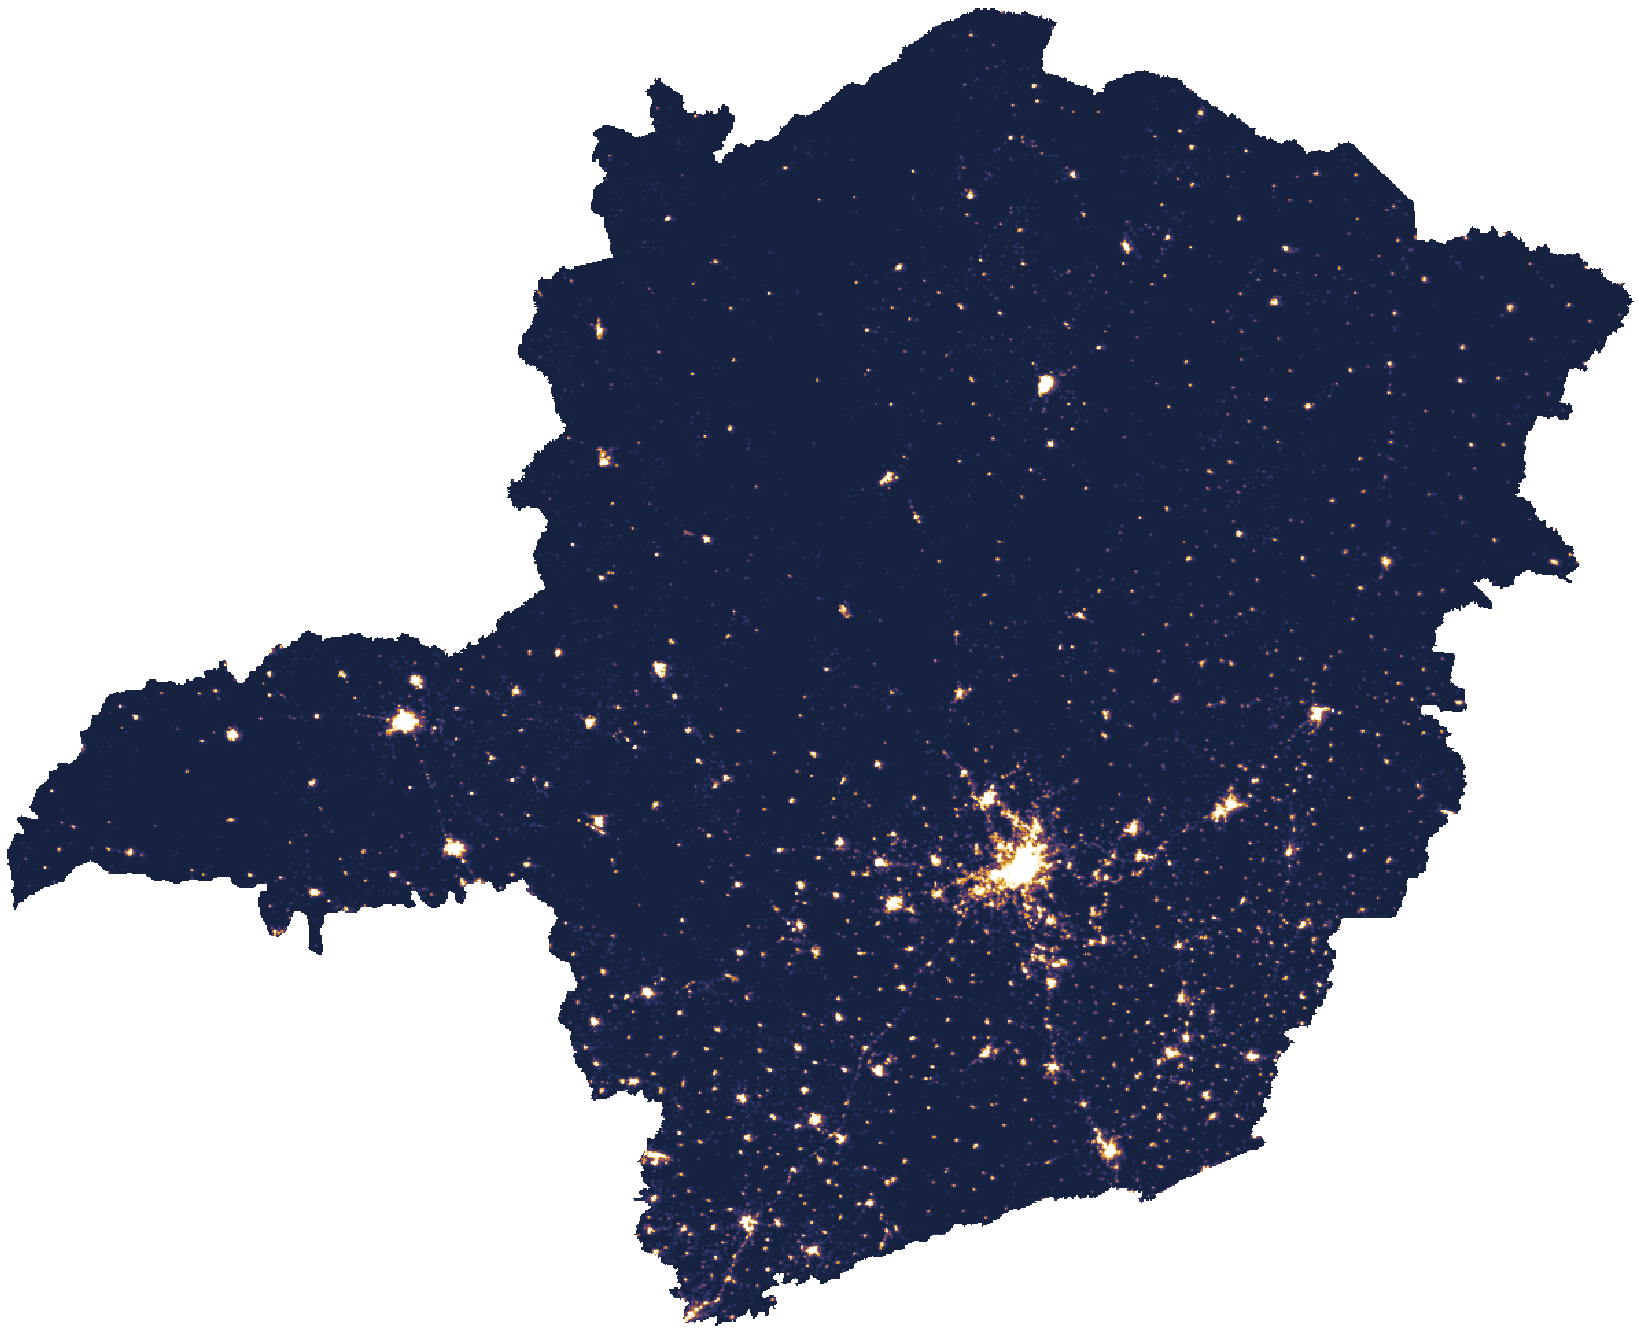
\includegraphics[height=0.96\paperheight]{hero_ntl.png}};
  \begin{scope}[x={($(map.south east)-(map.south west)$)},y={($(map.north west)-(map.south west)$)},shift={(map.south west)}]
    \draw[haze,line width=0.4pt] (0.625,0.345) -- (0.70,0.20) node[anchor=north west,inner sep=1pt,
      font=\fontsize{6.5}{8}\selectfont,text=haze] {Belo Horizonte};
    \draw[haze,line width=0.4pt] (0.245,0.465) -- (0.20,0.33) node[anchor=north,inner sep=1pt,
      font=\fontsize{6.5}{8}\selectfont,text=haze] {Uberlândia};
  \end{scope}
  \node[anchor=south east,font=\fontsize{6}{7}\selectfont,text=haze,align=right] at ($(current page.south east)+(-0.4,0.3)$)
    {VIIRS night lights 2022, one pixel per 1\,km cell};
\end{tikzpicture}
\begin{minipage}{0.47\textwidth}\raggedright
  \eyebrow[glow]{GIS term project \ $\cdot$ \ final presentation}\\[5pt]
  {\fontsize{10.5}{13}\selectfont\bfseries\color{glow}Geospatial Reasoning using LLMs and Generative AI\par}
  \vspace{8pt}
  {\blackfont\fontsize{21}{24}\selectfont\color{white}Reading the economy from space\par}
  \vspace{4pt}
  {\lightfont\fontsize{11}{14}\selectfont\color{white}Estimating municipal GDP from satellite embeddings, text and night lights, and putting it to use\par}
  \vspace{8pt}
  {\color{glow}\rule{1.6cm}{2.2pt}}\\[7pt]
  {\fontsize{10}{12}\selectfont\bfseries\color{white}Group 2}\\[4pt]
  {\fontsize{8.5}{12}\selectfont\color{white}Hemant \ {\color{haze}(22CS30029)}\\
   Saras Dipak Wagh \ {\color{haze}(22CS30048)}\\
   Pallav Agarwal \ {\color{haze}(22CS30040)}}\\[9pt]
  \href{https://github.com/chadsaras/GIS_Project}{\tikz[baseline=(b.base)]\node[fill=glow,rounded corners=3pt,inner xsep=6pt,
    inner ysep=4pt,font=\bfseries\fontsize{9}{11}\selectfont,text=night] (b)
    {\raisebox{-0.22em}{
\includegraphics[height=1.15em]{github_mark.png}}\ \ github.com/chadsaras/GIS\_Project};}
\end{minipage}
\end{frame}}

%======================== 2. PROBLEM ===================================
\setstage{1}
\begin{frame}{Local GDP is patchy; satellites see every place}
\begin{columns}[T,onlytextwidth]
\column{0.5\textwidth}
\centering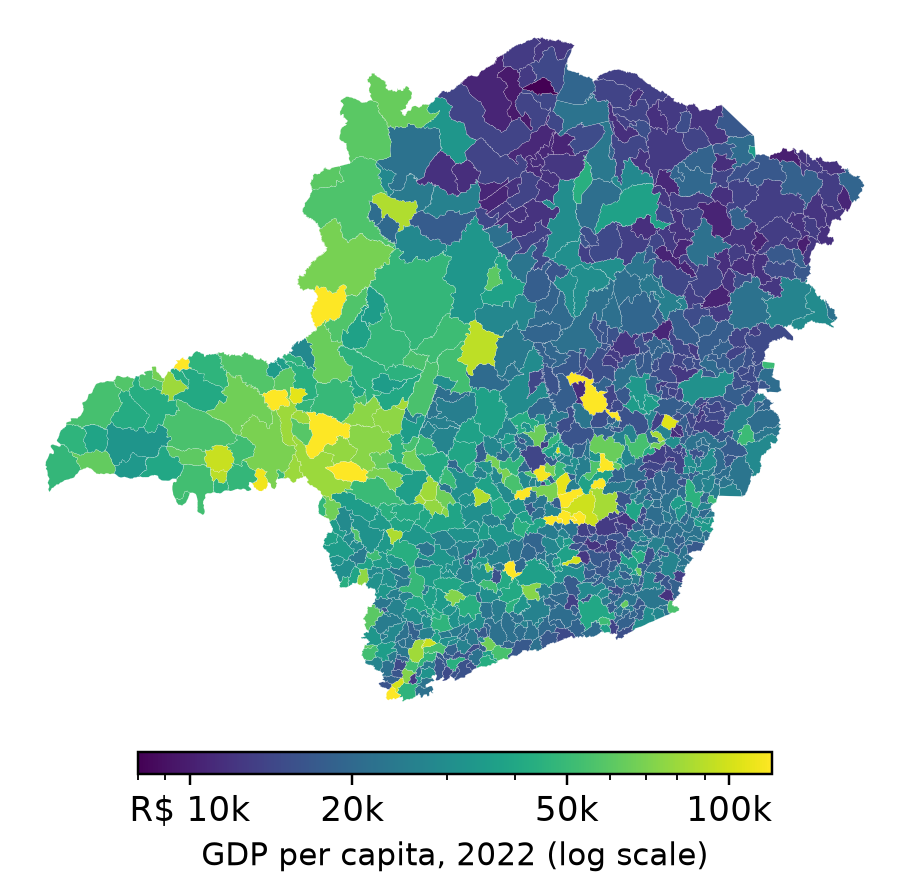
\includegraphics[height=5.5cm]{map_gdp.png}
\column{0.46\textwidth}
{\blackfont\fontsize{34}{36}\selectfont\color{cgdp}\nGdpRatio$\times$}\\[1pt]
{\footnotesize gap in GDP per capita inside one state:\\
\bfseries \nRichName{} \muted{(R\$\,\nRichGdp)} \ vs \ \nPoorName{} \muted{(R\$\,\nPoorGdp)}}\\[8pt]
\begin{itemize}\setlength{\itemsep}{3pt}\footnotesize
  \item Sub-national GDP is published \textbf{late}, \textbf{estimated} from partial data, or \textbf{missing} where statistics are weak.
  \item Satellites measure \textbf{every place, every year, with the same sensor}.
\end{itemize}
\vspace{8pt}
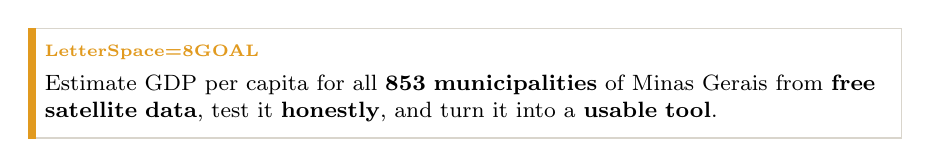
\begin{tikzpicture}
  \node[fill=white,draw=rule,text width=0.88\linewidth,inner sep=6pt,align=left,font=\footnotesize] (g)
    {\eyebrow[cntl]{Goal}\\[3pt]Estimate GDP per capita for all \textbf{\nMunis{} municipalities} of Minas Gerais from
     \textbf{free satellite data}, test it \textbf{honestly}, and turn it into a \textbf{usable tool}.};
  \fill[cntl] (g.north west) rectangle ($(g.south west)+(3pt,0)$);
\end{tikzpicture}
\end{columns}
\end{frame}

%======================== 3. SINCE THE MID-TERM ========================
\begin{frame}{Since the mid-term: from first results to a tested application}
\centering
{\renewcommand{\arraystretch}{1.3}\footnotesize
\begin{tabular}{@{}L{4.6cm}@{\hspace{6pt}}c@{\hspace{6pt}}L{6.6cm}@{}}
\eyebrow{At the mid-term (6 Oct)} & & \eyebrow[okc]{Final (November)}\\[-2pt]
\chip{muted}{DONE} \ Models V1--V12, RQ1--RQ4 answered & {\color{glow}$\rightarrow$} & \chip{okc}{NEW} \ \textbf{Same answers after a full rerun} from scratch\\
\chip{muted}{RUNNING} \ Caption audit & {\color{glow}$\rightarrow$} & \chip{okc}{DONE} \ \textbf{\nAuditRaw{} of AI captions} hold a false claim; checks cut it to \nAuditClean\\
\chip{muted}{CODE READY} \ Error analysis (RQ5) & {\color{glow}$\rightarrow$} & \chip{okc}{DONE} \ \textbf{Mines, steel mills, commuter towns} are invisible from space\\
\chip{muted}{MISSING} \ Uncertainty & {\color{glow}$\rightarrow$} & \chip{okc}{NEW} \ \textbf{Honest 90\% ranges} (\nCovNinety{} held) and a risk warning\\
\chip{muted}{MISSING} \ Test outside the study area & {\color{glow}$\rightarrow$} & \chip{okc}{NEW} \ \textbf{São Paulo transfer}: satellites travel, night lights do not\\
\chip{muted}{MISSING} \ Application & {\color{glow}$\rightarrow$} & \chip{okc}{NEW} \ \textbf{Web application}: estimates where statistics are missing\\
\end{tabular}}\par\vspace{10pt}
\fnote{Also: a 12-page report, a one-command rerun of the whole pipeline, and checks of ideas that did not work (slide 16).}
\end{frame}

%======================== 4. TWO IDEAS =================================
\setstage{2}
\begin{frame}{Two recent ideas, never tested together}
\centering
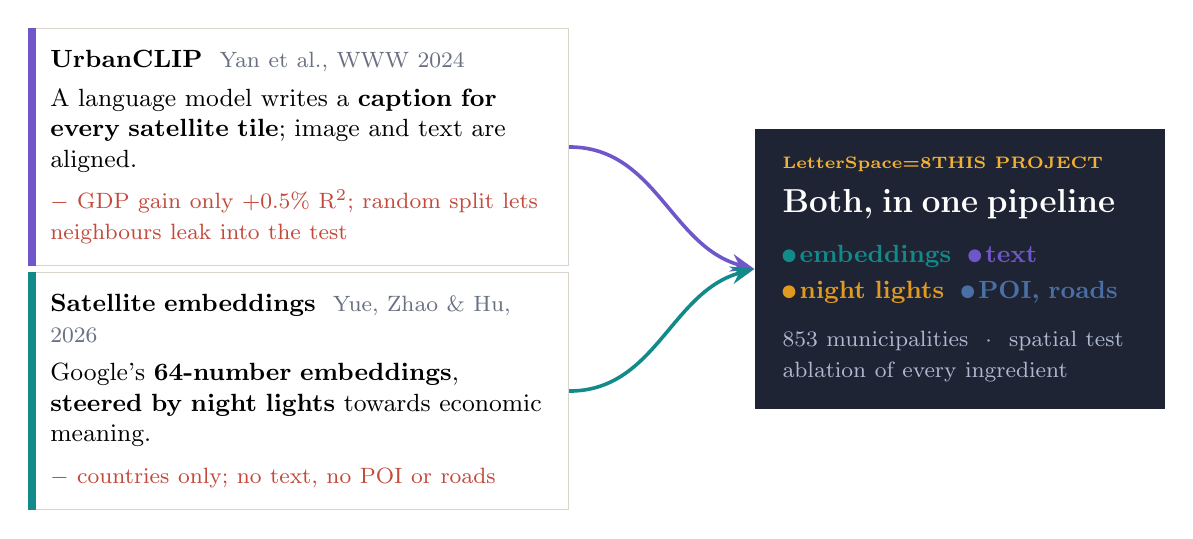
\begin{tikzpicture}[
  card/.style={fill=white,draw=rule,text width=6.3cm,inner sep=8pt,align=left,font=\small},
  arr/.style={-{Stealth[length=3mm]},line width=1.3pt}]
  \node[card] (u) at (0,1.55) {{\bfseries UrbanCLIP} \ \muted{\footnotesize Yan et al., WWW 2024}\\[3pt]
    A language model writes a \textbf{caption for every satellite tile}; image and text are aligned.\\[4pt]
    {\footnotesize\color{cgdp}$-$\ GDP gain only +0.5\% R\textsuperscript{2}; random split lets neighbours leak into the test}};
  \fill[ctxt] (u.north west) rectangle ($(u.south west)+(3pt,0)$);
  \node[card] (e) at (0,-1.55) {{\bfseries Satellite embeddings} \ \muted{\footnotesize Yue, Zhao \& Hu, 2026}\\[3pt]
    Google's \textbf{64-number embeddings}, \textbf{steered by night lights} towards economic meaning.\\[4pt]
    {\footnotesize\color{cgdp}$-$\ countries only; no text, no POI or roads}};
  \fill[cimg] (e.north west) rectangle ($(e.south west)+(3pt,0)$);
  \node[fill=ink,text=white,text width=4.5cm,inner sep=10pt,align=left,font=\small] (o) at (8.4,0)
    {\eyebrow[glow]{This project}\\[5pt]
     {\large\bfseries Both, in one pipeline}\\[7pt]
     \ing{cimg}{embeddings} \ \ing{ctxt}{text}\\[2pt]
     \ing{cntl}{night lights} \ \ing{cpoi}{POI, roads}\\[8pt]
     {\color{haze}\footnotesize \nMunis{} municipalities \ $\cdot$ \ spatial test\\ablation of every ingredient}};
  \draw[arr,ctxt] (u.east) to[out=0,in=165] (o.west);
  \draw[arr,cimg] (e.east) to[out=0,in=195] (o.west);
\end{tikzpicture}
\end{frame}

%======================== 5. PIPELINE ==================================
\begin{frame}{Three learning stages, from no labels to official GDP}
\centering
\begin{tikzpicture}[
  thumbcap/.style={font=\fontsize{7}{8.5}\selectfont,align=center,text=ink,inner sep=1pt},
  flow/.style={-{Stealth[length=2.6mm]},line width=1.4pt,draw=ink}]
  \node[stage=ctxt] (A) at (0,0) {\eyebrow[ctxt]{Stage A}\\[2pt]{\bfseries\small Image--text alignment}\\[1pt]embeddings and captions pulled together};
  \node[stage=cntl] (B) at (4.1,0) {\eyebrow[cntl]{Stage B}\\[2pt]{\bfseries\small Night-light steering}\\[1pt]predict each cell's light, keep the inner layer};
  \node[stage=cgdp] (C) at (8.2,0) {\eyebrow[cgdp]{Stage C}\\[2pt]{\bfseries\small Add up the cells}\\[1pt]per municipality, then predict};
  \node[fill=ink,text=white,text width=2.3cm,minimum height=1.6cm,align=center,inner sep=5pt,font=\footnotesize] (Y) at (11.95,0)
    {{\bfseries\small log GDP\\per capita}\\[2pt]{\color{haze}\nMunis{} municipalities}};
  \draw[flow] (A) -- (B); \draw[flow] (B) -- (C); \draw[flow] (C) -- (Y);
  \node[inner sep=0] (ti) at (-1.0,2.4) {\framed{cimg}{height=1.2cm}{layer_gsed.png}};
  \node[inner sep=0] (tc) at (1.0,2.4) {\framed{ctxt}{height=1.2cm}{caption_tile.png}};
  \node[inner sep=0] (tn) at (4.1,2.4) {\framed{cntl}{height=1.2cm}{layer_ntl.png}};
  \node[inner sep=0] (tg) at (8.2,2.4) {\framed{cgdp}{height=1.2cm}{layer_gdp.png}};
  \node[thumbcap,above=1pt of ti] {\bfseries embeddings};
  \node[thumbcap,above=1pt of tc] {\bfseries captions + facts};
  \node[thumbcap,above=1pt of tn] {\bfseries night lights};
  \node[thumbcap,above=1pt of tg] {\bfseries official GDP};
  \draw[feed=cimg] (ti.south) -- ($(A.north)+(-1.0,0)$);
  \draw[feed=ctxt] (tc.south) -- ($(A.north)+(1.0,0)$);
  \draw[feed=cntl] (tn) -- (B);
  \draw[feed=cgdp] (tg) -- (C);
  \foreach \n/\t/\c in {A/no labels/ctxt,B/cheap proxy label/cntl,C/853 real labels/cgdp}
    \node[below=4pt of \n,font=\bfseries\fontsize{6.5}{8}\selectfont,text=\c] {\MakeUppercase{\t}};
\end{tikzpicture}
\vspace{4pt}

\fnote{Captions are needed only in training: at prediction time each cell uses its embedding alone, so any place can be estimated.}
\end{frame}

%======================== 6. DATA ======================================
\begin{frame}{Six free layers on one 1\,km grid}
\begin{columns}[c,onlytextwidth]
\column{0.68\textwidth}
\begin{tikzpicture}[
  lname/.style={anchor=west,font=\footnotesize\bfseries,inner sep=0},
  lsrc/.style={anchor=north west,font=\fontsize{6.5}{8}\selectfont,text=muted,inner sep=0,yshift=-2pt}]
  \foreach \img/\c/\name/\src [count=\i from 0] in {
      gsed/cimg/Satellite embeddings/{Google GSED, 64 numbers, 10\,m to 1\,km},
      captions/ctxt/Captioned tiles/{\nCaptions{} Esri tiles, Qwen2.5-VL},
      buildings/ink/Buildings/{Microsoft + OSM footprints},
      roads/cpoi/Roads and POIs/{OpenStreetMap},
      ntl/cntl/Night lights/{VIIRS 2022},
      gdp/cgdp/GDP per capita (target)/{IBGE 2022, official}} {
    \begin{scope}[yshift=\i*0.74cm,cm={1,0.28,-0.62,0.5,(0,0)}]
      \fill[white,draw=\c,line width=0.8pt] (0,0) rectangle (3.0,2.44);
      \node[transform shape,anchor=south west,inner sep=0] at (0,0) {\includegraphics[width=3.0cm,height=2.44cm]{layer_\img.png}};
      \coordinate (r\i) at (3.0,1.22);
    \end{scope}
    \draw[\c,line width=0.5pt] (r\i) -- (r\i -| 4.0,0);
    \fill[\c] (r\i -| 4.0,0) circle (1.5pt);
    \node[lname,text=\c] (n\i) at ($(r\i -| 4.0,0)+(0.15,0.07)$) {\name};
    \node[lsrc] at (n\i.south west) {\src};
  }
\end{tikzpicture}
\column{0.3\textwidth}
\kpi{ink}{\nMunis}{municipalities}\\[6pt]
\kpi{ink}{\nCells}{1\,km cells}\\[6pt]
\kpi{ctxt}{\nCaptions}{captioned tiles}\\[6pt]
\kpi{ink}{\nBuildings}{building footprints}\\[8pt]
\fnote{All layers free and aligned on the same grid (EPSG:31983). The target is official statistics, not night lights.}
\end{columns}
\end{frame}

%======================== 7. CAPTIONS + AUDIT ==========================
\begin{frame}{AI captions help, but a third of them contain a false claim}
\begin{columns}[T,onlytextwidth]
\column{0.25\textwidth}
\begin{tikzpicture}
  \node[inner sep=0] (im) {\framed{ctxt}{width=\linewidth}{caption_tile.png}};
  \begin{scope}[x={($(im.south east)-(im.south west)$)},y={($(im.north west)-(im.south west)$)},shift={(im.south west)}]
    \draw[cgdp,line width=1.3pt,dashed] (0.43,0.64) ellipse (0.36 and 0.33);
    \node[anchor=south west,font=\fontsize{6}{7}\selectfont\bfseries,fill=white,text=cgdp,inner sep=2pt,text width=0.86\linewidth]
      at (0.03,0.03) {centre-pivot irrigation, not a mine};
  \end{scope}
\end{tikzpicture}\\[2pt]
\fnote{Esri World Imagery, about 1\,m per pixel}
\column{0.37\textwidth}
\eyebrow[ctxt]{Qwen2.5-VL-7B caption, after the checks}\\[-2pt]
\begin{itemize}\setlength{\itemsep}{1pt}\fontsize{7.2}{8.6}\selectfont
\dropped{The satellite image shows a large circular area with concentric rings, likely a mine pit, surrounded by a grid of smaller rectangular plots of farmland.}{unsupported industry claim}
\keep{Roads crisscross the area, connecting the plots and the perimeter.}
\keep{Vegetation is sparse, mostly along the edges and in some patches within the farmland.}
\keep{A small body of water, possibly a pond, is visible near the farmland.}
\keep{No buildings or industrial structures are evident, suggesting minimal built-up area.}
\dropped{The overall scene appears to be an agricultural landscape with a focus on farming and possibly mining operations.}{filler}

\end{itemize}
\fnote{Checks against land cover, roads and building footprints keep \nKept{} of \nSentences{} sentences.}
\column{0.34\textwidth}
\eyebrow{Blind audit of 300 captions}\\[6pt]
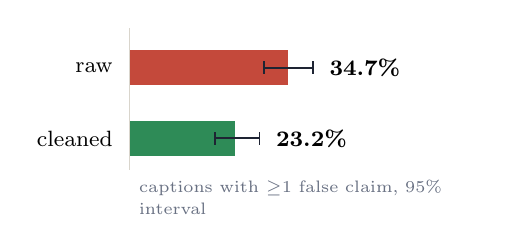
\begin{tikzpicture}[x=0.058cm,y=1cm]
  \foreach \v/\lo/\hi/\lab/\c [count=\i] in {34.7/29.5/40.2/raw/cgdp,23.2/18.7/28.5/cleaned/okc} {
    \node[anchor=east,font=\footnotesize] at (-1.5,-\i*0.9) {\lab};
    \fill[\c] (0,-\i*0.9-0.22) rectangle (\v,-\i*0.9+0.22);
    \draw[ink,line width=0.7pt] (\lo,-\i*0.9) -- (\hi,-\i*0.9);
    \draw[ink,line width=0.7pt] (\lo,-\i*0.9-0.08) -- ++(0,0.16); \draw[ink,line width=0.7pt] (\hi,-\i*0.9-0.08) -- ++(0,0.16);
    \node[anchor=west,font=\bfseries\footnotesize] at (\hi+1.5,-\i*0.9) {\v\%};
  }
  \draw[rule] (0,-0.4) -- (0,-2.2);
  \node[font=\fontsize{6.5}{8}\selectfont,text=muted,anchor=north west,text width=4.3cm] at (0,-2.2)
    {captions with $\geq$1 false claim, 95\% interval};
\end{tikzpicture}\\[4pt]
{\fontsize{7.5}{9}\selectfont Cleaning removes \textbf{\nAuditRecall} of false sentences; \textbf{\nAuditPrecision} of what it removes is false or vague.}\\[3pt]
\fnote{Labelled by an LLM (Claude) from each tile; a human check is still open.}
\end{columns}
\end{frame}

%======================== 8. TEST ======================================
\setstage{3}
\begin{frame}{Every municipality is tested in a region never seen}
\begin{columns}[c,onlytextwidth]
\column{0.47\textwidth}
\centering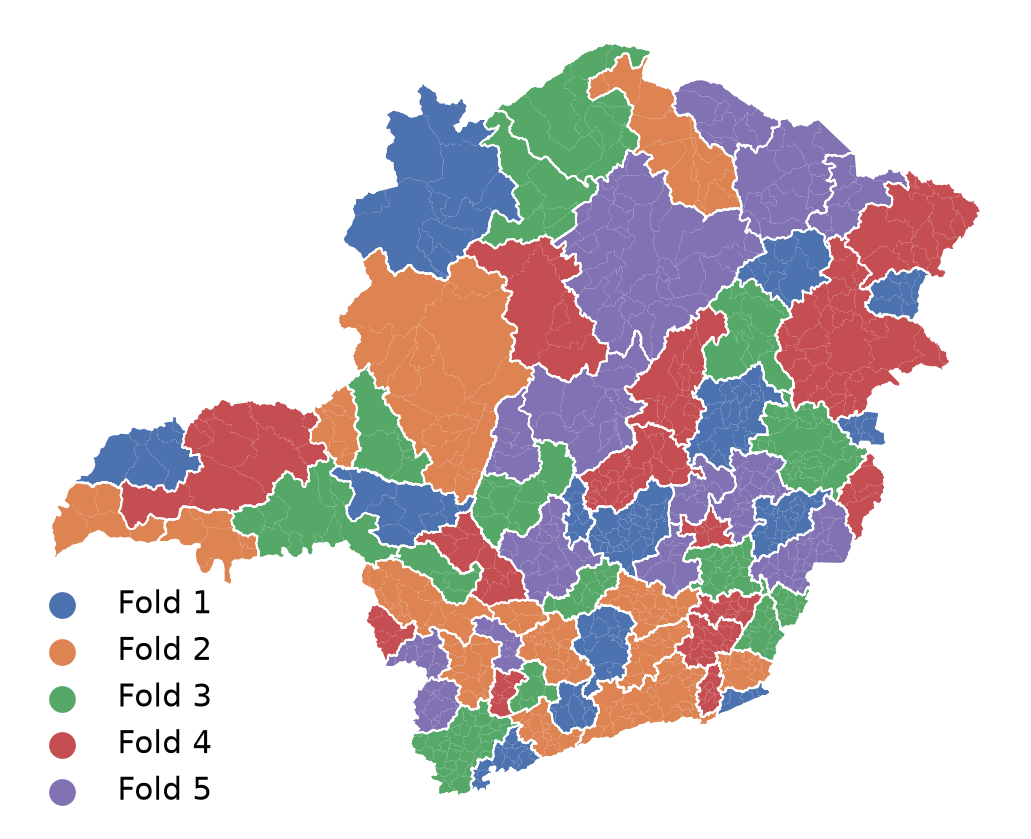
\includegraphics[height=5.3cm]{map_folds.png}\\[-2pt]
\fnote{70 official regions (white outlines) grouped into 5 folds}
\column{0.5\textwidth}
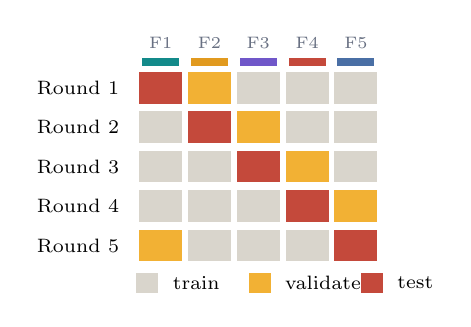
\begin{tikzpicture}[x=0.62cm,y=0.5cm]
  \foreach \c [count=\f from 0] in {cimg,cntl,ctxt,cgdp,cpoi} {
    \fill[\c] (\f+0.12,0.55) rectangle (\f+0.88,0.75);
    \node[font=\fontsize{6.5}{8}\selectfont,text=muted] at (\f+0.5,1.15) {F\the\numexpr\f+1\relax};
  }
  \foreach \r in {0,...,4} {
    \node[anchor=east,font=\fontsize{7}{8}\selectfont] at (-0.15,-\r) {Round \the\numexpr\r+1\relax};
    \pgfmathtruncatemacro\v{mod(\r+1,5)}
    \foreach \f in {0,...,4} {
      \ifnum\f=\r \def\fc{cgdp}\else\ifnum\f=\v \def\fc{glow}\else\def\fc{rule}\fi\fi
      \fill[\fc] (\f+0.06,-\r-0.4) rectangle (\f+0.94,-\r+0.4);
    }
  }
  \foreach \c/\t [count=\k from 0] in {rule/train,glow/validate,cgdp/test} {
    \fill[\c] (\k*2.3,-5.2) rectangle ++(0.45,0.5);
    \node[anchor=west,font=\fontsize{7}{8}\selectfont] at (\k*2.3+0.55,-4.95) {\t};
  }
\end{tikzpicture}\\[8pt]
\begin{itemize}\setlength{\itemsep}{3pt}\footnotesize
  \item Whole regions held out: \textbf{no look-alike neighbour} in training. All stages retrained each round.
  \item The same rule holds for every range, warning and choice shown later: \textbf{nothing is tuned on test towns}.
\end{itemize}
\vspace{2pt}
\fnote{Models are compared on the same folds with a block bootstrap over regions (95\% intervals).}
\end{columns}
\end{frame}

%======================== 9. RESULTS ===================================
\setstage{4}
\begin{frame}{Satellites explain half of GDP gaps, twice night lights}
\begin{columns}[c,onlytextwidth]
\column{0.62\textwidth}
\resizebox{!}{5.2cm}{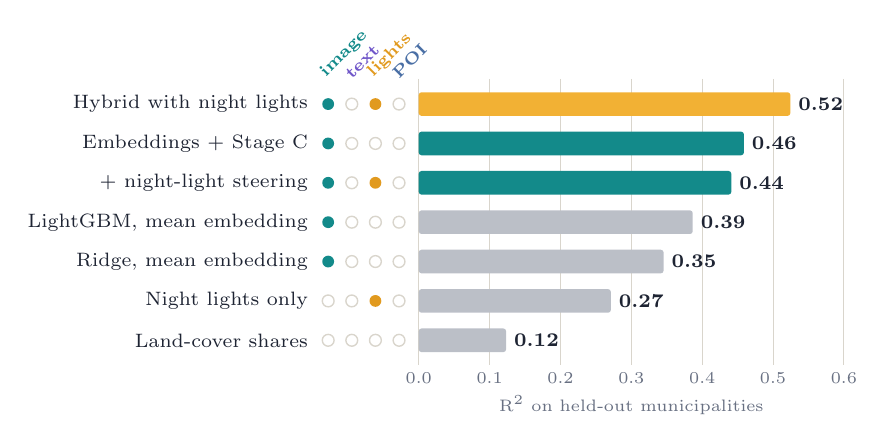
\begin{tikzpicture}[x=1cm,y=1cm,
  lab/.style={font=\fontsize{7.5}{9}\selectfont,text=ink,inner sep=0pt},
  num/.style={font=\bfseries\fontsize{7.5}{9}\selectfont,inner sep=1pt},
  tick/.style={font=\fontsize{6.5}{7.8}\selectfont,text=muted,inner sep=0pt}]
\node[tick,text=cimg,font=\bfseries\fontsize{6}{7}\selectfont,rotate=45,anchor=south west] at (-1.15,0.3) {image};
\node[tick,text=ctxt,font=\bfseries\fontsize{6}{7}\selectfont,rotate=45,anchor=south west] at (-0.85,0.3) {text};
\node[tick,text=cntl,font=\bfseries\fontsize{6}{7}\selectfont,rotate=45,anchor=south west] at (-0.55,0.3) {lights};
\node[tick,text=cpoi,font=\bfseries\fontsize{6}{7}\selectfont,rotate=45,anchor=south west] at (-0.25,0.3) {POI};
\draw[rule,line width=0.4pt] (0.00,0.32) -- (0.00,-3.32);
\node[tick,anchor=north] at (0.00,-3.40) {0.0};
\draw[rule,line width=0.4pt] (0.90,0.32) -- (0.90,-3.32);
\node[tick,anchor=north] at (0.90,-3.40) {0.1};
\draw[rule,line width=0.4pt] (1.80,0.32) -- (1.80,-3.32);
\node[tick,anchor=north] at (1.80,-3.40) {0.2};
\draw[rule,line width=0.4pt] (2.70,0.32) -- (2.70,-3.32);
\node[tick,anchor=north] at (2.70,-3.40) {0.3};
\draw[rule,line width=0.4pt] (3.60,0.32) -- (3.60,-3.32);
\node[tick,anchor=north] at (3.60,-3.40) {0.4};
\draw[rule,line width=0.4pt] (4.50,0.32) -- (4.50,-3.32);
\node[tick,anchor=north] at (4.50,-3.40) {0.5};
\draw[rule,line width=0.4pt] (5.40,0.32) -- (5.40,-3.32);
\node[tick,anchor=north] at (5.40,-3.40) {0.6};
\node[tick,anchor=north] at (2.70,-3.70) {R\textsuperscript{2} on held-out municipalities};
\node[lab,anchor=east] at (-1.4,-0.00) {Hybrid with night lights};
\path[fill=cimg] (-1.15,-0.00) circle (0.075);
\path[draw=rule,line width=0.5pt,fill=white] (-0.85,-0.00) circle (0.075);
\path[fill=cntl] (-0.55,-0.00) circle (0.075);
\path[draw=rule,line width=0.5pt,fill=white] (-0.25,-0.00) circle (0.075);
\fill[glow,rounded corners=1pt] (0,-0.15) rectangle (4.72,0.15);
\node[num,anchor=west,text=ink] at (4.78,-0.00) {0.52};
\node[lab,anchor=east] at (-1.4,-0.50) {Embeddings + Stage C};
\path[fill=cimg] (-1.15,-0.50) circle (0.075);
\path[draw=rule,line width=0.5pt,fill=white] (-0.85,-0.50) circle (0.075);
\path[draw=rule,line width=0.5pt,fill=white] (-0.55,-0.50) circle (0.075);
\path[draw=rule,line width=0.5pt,fill=white] (-0.25,-0.50) circle (0.075);
\fill[cimg,rounded corners=1pt] (0,-0.65) rectangle (4.13,-0.35);
\node[num,anchor=west,text=ink] at (4.19,-0.50) {0.46};
\node[lab,anchor=east] at (-1.4,-1.00) {+ night-light steering};
\path[fill=cimg] (-1.15,-1.00) circle (0.075);
\path[draw=rule,line width=0.5pt,fill=white] (-0.85,-1.00) circle (0.075);
\path[fill=cntl] (-0.55,-1.00) circle (0.075);
\path[draw=rule,line width=0.5pt,fill=white] (-0.25,-1.00) circle (0.075);
\fill[cimg,rounded corners=1pt] (0,-1.15) rectangle (3.97,-0.85);
\node[num,anchor=west,text=ink] at (4.03,-1.00) {0.44};
\node[lab,anchor=east] at (-1.4,-1.50) {LightGBM, mean embedding};
\path[fill=cimg] (-1.15,-1.50) circle (0.075);
\path[draw=rule,line width=0.5pt,fill=white] (-0.85,-1.50) circle (0.075);
\path[draw=rule,line width=0.5pt,fill=white] (-0.55,-1.50) circle (0.075);
\path[draw=rule,line width=0.5pt,fill=white] (-0.25,-1.50) circle (0.075);
\fill[muted!45,rounded corners=1pt] (0,-1.65) rectangle (3.48,-1.35);
\node[num,anchor=west,text=ink] at (3.54,-1.50) {0.39};
\node[lab,anchor=east] at (-1.4,-2.00) {Ridge, mean embedding};
\path[fill=cimg] (-1.15,-2.00) circle (0.075);
\path[draw=rule,line width=0.5pt,fill=white] (-0.85,-2.00) circle (0.075);
\path[draw=rule,line width=0.5pt,fill=white] (-0.55,-2.00) circle (0.075);
\path[draw=rule,line width=0.5pt,fill=white] (-0.25,-2.00) circle (0.075);
\fill[muted!45,rounded corners=1pt] (0,-2.15) rectangle (3.11,-1.85);
\node[num,anchor=west,text=ink] at (3.17,-2.00) {0.35};
\node[lab,anchor=east] at (-1.4,-2.50) {Night lights only};
\path[draw=rule,line width=0.5pt,fill=white] (-1.15,-2.50) circle (0.075);
\path[draw=rule,line width=0.5pt,fill=white] (-0.85,-2.50) circle (0.075);
\path[fill=cntl] (-0.55,-2.50) circle (0.075);
\path[draw=rule,line width=0.5pt,fill=white] (-0.25,-2.50) circle (0.075);
\fill[muted!45,rounded corners=1pt] (0,-2.65) rectangle (2.44,-2.35);
\node[num,anchor=west,text=ink] at (2.50,-2.50) {0.27};
\node[lab,anchor=east] at (-1.4,-3.00) {Land-cover shares};
\path[draw=rule,line width=0.5pt,fill=white] (-1.15,-3.00) circle (0.075);
\path[draw=rule,line width=0.5pt,fill=white] (-0.85,-3.00) circle (0.075);
\path[draw=rule,line width=0.5pt,fill=white] (-0.55,-3.00) circle (0.075);
\path[draw=rule,line width=0.5pt,fill=white] (-0.25,-3.00) circle (0.075);
\fill[muted!45,rounded corners=1pt] (0,-3.15) rectangle (1.11,-2.85);
\node[num,anchor=west,text=ink] at (1.17,-3.00) {0.12};
\end{tikzpicture}
}\\[2pt]
\fnote{Dots: ingredients each model uses. Hybrid = best model blended with night lights.}
\column{0.34\textwidth}
{\blackfont\fontsize{24}{26}\selectfont\color{ink}\nHybridR}\ \ {\fontsize{7.5}{9}\selectfont\color{muted}R\textsuperscript{2}, hybrid, unseen regions}\\[2pt]
\chip{okc}{CONFIRMED BY A FULL RERUN}\\[7pt]
\chip{ctxt}{RQ2 \ TEXT} \ {\footnotesize\bfseries small gain, not robust}\\[-1pt]\fnote{$\Delta$RMSE \nRerunTextFrozen, rerun \nRerunTextNew; intervals include 0}\\[5pt]
\chip{muted}{RQ1 \ STEERING} \ {\footnotesize\bfseries no clear effect}\\[-1pt]\fnote{\RQone}\\[5pt]
\chip{muted}{RQ3 \ POI, ROADS} \ {\footnotesize\bfseries nothing added}\\[-1pt]\fnote{\RQthree}\\[5pt]
\chip{cntl}{RQ4 \ HYBRID} \ {\footnotesize\bfseries best, not significant}\\[-1pt]\fnote{\RQfour}\\[4pt]
\fnote{RMSE differences (log GDP per capita), 95\% intervals; negative = first model better.}
\end{columns}
\end{frame}

%======================== 10. MAPS =====================================
\begin{frame}{Predictions follow the map, but are pulled towards the middle}
\begin{columns}[T,onlytextwidth]
\column{0.28\textwidth}\centering
\eyebrow[cgdp]{Official}\\[2pt]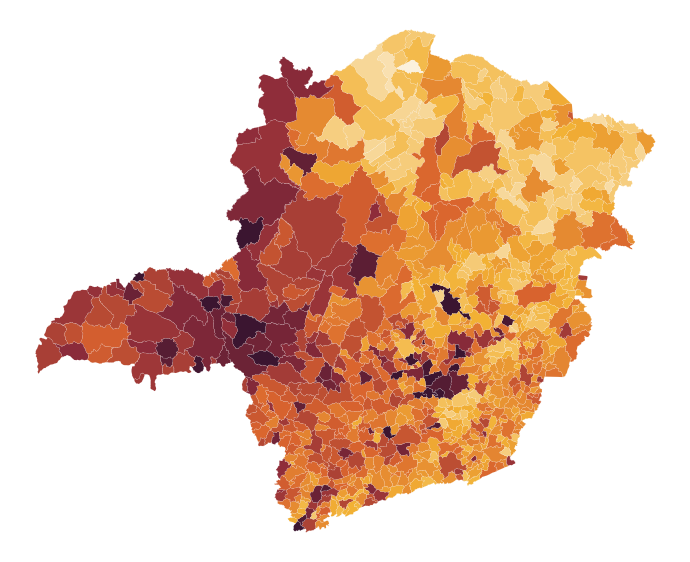
\includegraphics[width=\linewidth]{map_official.png}
\column{0.28\textwidth}\centering
\eyebrow[cgdp]{Predicted (hybrid)}\\[2pt]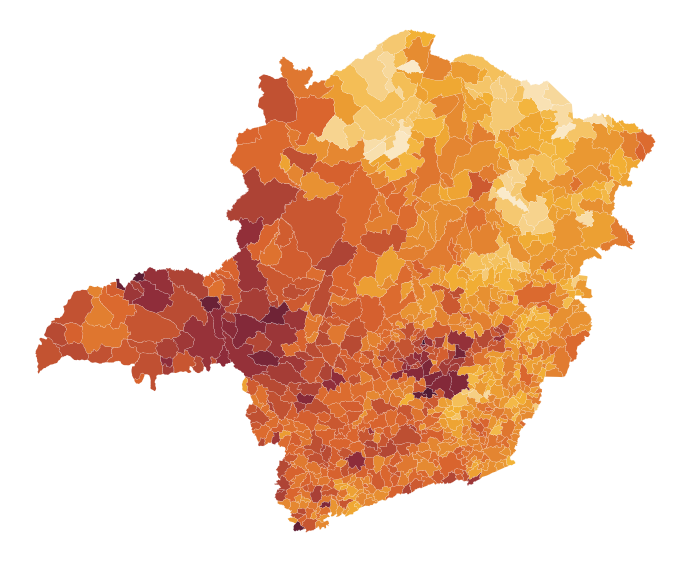
\includegraphics[width=\linewidth]{map_predicted.png}
\column{0.28\textwidth}\centering
\eyebrow{Error}\\[2pt]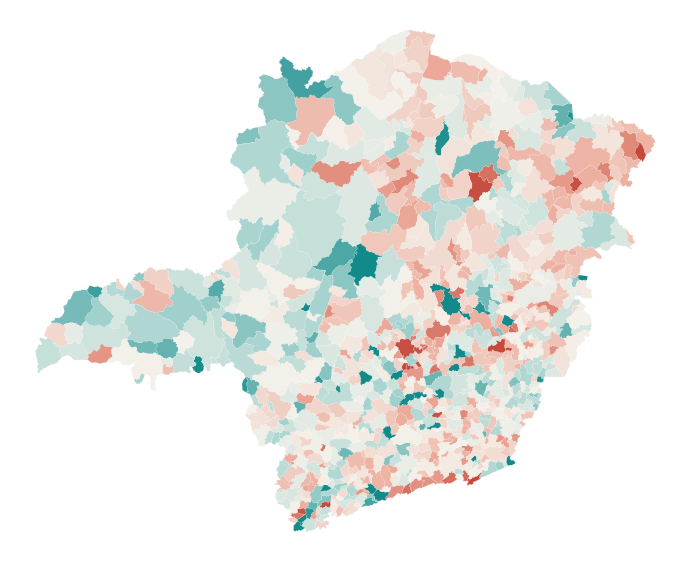
\includegraphics[width=\linewidth]{map_error.png}
\column{0.12\textwidth}
\end{columns}
\begin{columns}[T,onlytextwidth]
\column{0.56\textwidth}\centering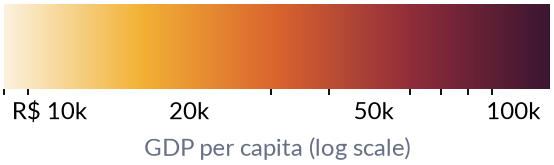
\includegraphics[width=0.5\linewidth]{cbar_gdp.png}
\column{0.28\textwidth}\centering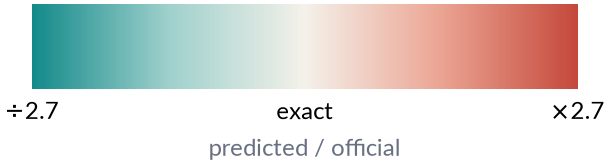
\includegraphics[width=0.85\linewidth]{cbar_err.png}
\column{0.12\textwidth}
\end{columns}
\vspace{8pt}
\begin{columns}[T,onlytextwidth]
\column{0.24\textwidth}
{\blackfont\fontsize{20}{22}\selectfont\color{ink}\nWithinHalf}\\{\fontsize{7}{8.5}\selectfont\color{muted}of municipalities predicted within a factor 1.5 of official}
\column{0.74\textwidth}
\footnotesize \textcolor{cimg}{\textbf{Under-predicted:}} rich agribusiness and mining towns (west, centre).\\[2pt]
\textcolor{cgdp}{\textbf{Over-predicted:}} small public-sector and commuter towns.
\end{columns}
\end{frame}

%======================== 11. RQ5: THE BIG MISSES =======================
\setstage{5}
\begin{frame}{The biggest misses are mines and steel mills satellites cannot see}
\begin{columns}[c,onlytextwidth]
\column{0.5\textwidth}
\centering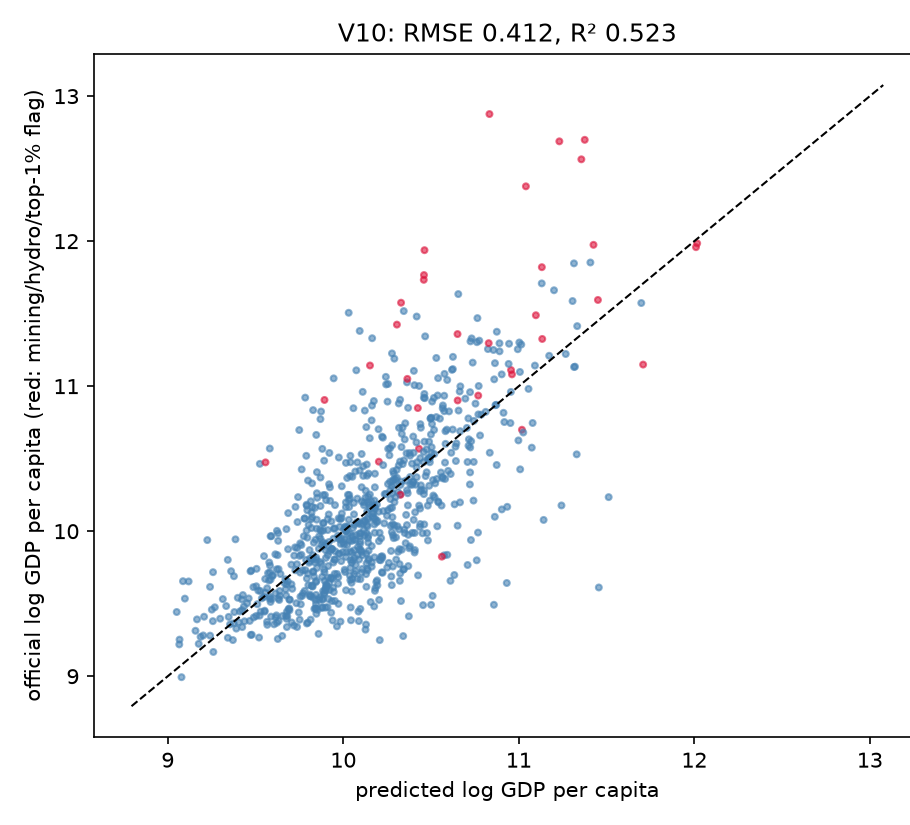
\includegraphics[height=5.0cm]{scatter_v10.png}\\[-1pt]
\fnote{Hybrid, 853 test predictions; red = flagged mining or hydro.}
\column{0.47\textwidth}
\eyebrow{Ten largest gaps}\\[2pt]
{\renewcommand{\arraystretch}{1.0}\fontsize{7.5}{9}\selectfont
\begin{tabular}{@{}lrl@{}}
\toprule
Municipality & gap & likely reason \\
\midrule
Catas Altas & $-2.04$ & {\color{cimg}\bfseries iron-ore mine} \\
Santa Cruz de Minas & $+1.84$ & {\color{cgdp}\bfseries tiny commuter town} \\
Ressaquinha & $-1.48$ & {\color{cimg}\bfseries large plant} \\
Conceição do Mato Dentro & $-1.48$ & {\color{cimg}\bfseries iron-ore mine} \\
S.\ Gonçalo do Rio Abaixo & $-1.46$ & {\color{cimg}\bfseries iron-ore mine} \\
Mário Campos & $+1.37$ & {\color{cgdp}\bfseries BH commuter town} \\
Itatiaiuçu & $-1.34$ & {\color{cimg}\bfseries iron-ore mine} \\
Extrema & $-1.32$ & {\color{cimg}\bfseries logistics hub} \\
Ouro Branco & $-1.31$ & {\color{cimg}\bfseries steel mill} \\
Chiador & $+1.29$ & {\color{cgdp}\bfseries public-sector town} \\
\bottomrule
\end{tabular}}\\[3pt]
\fnote{Gap = predicted $-$ official (log). A few cells make most of the output. Reasons are candidates.}
\end{columns}
\end{frame}

%======================== 12. RQ5: ERROR STRUCTURE =====================
\begin{frame}{Errors grow with income, but half as fast as with night lights}
\begin{columns}[c,onlytextwidth]
\column{0.5\textwidth}
\centering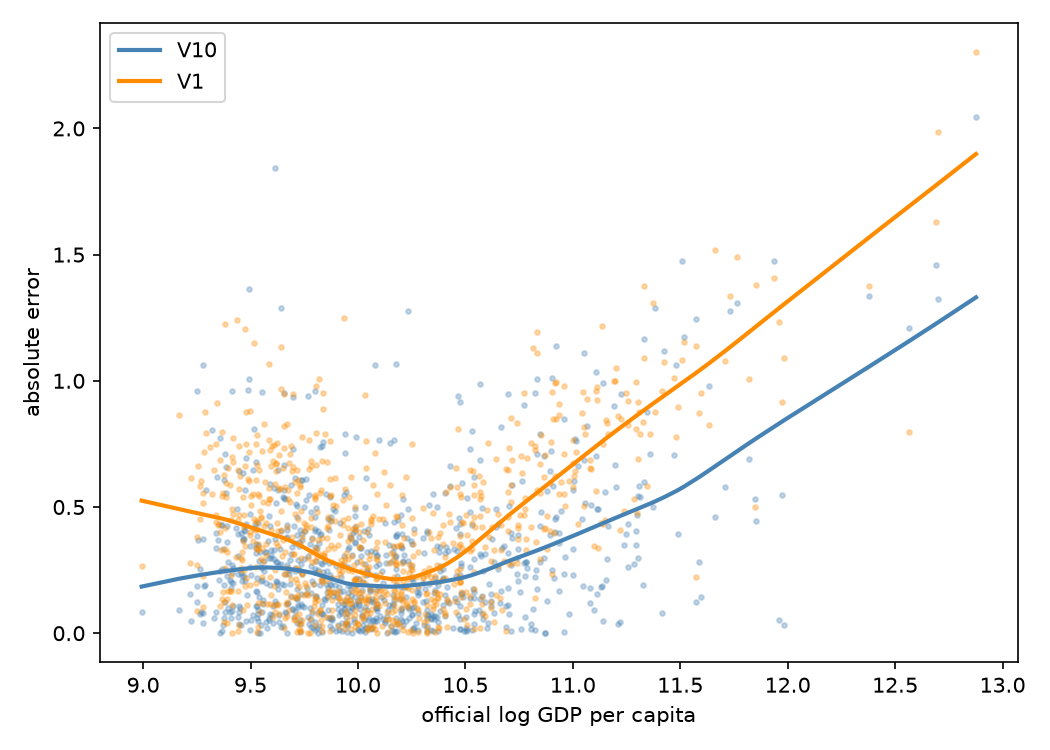
\includegraphics[width=\linewidth]{error_vs_income.png}\\[-2pt]
\fnote{Absolute error against official income, LOWESS. Blue: hybrid; orange: night lights only.}
\column{0.46\textwidth}
\kpi{ink}{\nSlopeV{} \ {\fontsize{12}{14}\selectfont\color{muted}vs} \ \nSlopeNtl}{extra error per log point of income, hybrid vs night lights}\\[8pt]
\kpi{ink}{\nMoranV{} \ {\fontsize{12}{14}\selectfont\color{muted}vs} \ \nMoranNtl}{Moran's I of errors: still clustered, half as much}\\[8pt]
\kpi{cgdp}{$\rho = \nUncRho$}{spread across training seeds does not predict error: seeds are not a confidence interval}\\[8pt]
\fnote{Error regression with region-clustered SEs: errors rise with income and built-up share, fall with services share;
OSM completeness does not matter. This is why the application needs its own honest ranges (next).}
\end{columns}
\end{frame}

%======================== 13. RELIABILITY ===============================
\setstage{6}
\begin{frame}{Every estimate ships with an honest range and a warning}
\begin{columns}[T,onlytextwidth]
\column{0.4\textwidth}
\eyebrow{Ranges: promised vs achieved}\\[6pt]
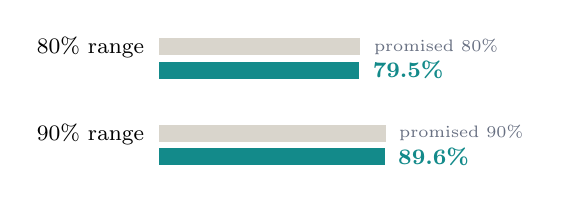
\begin{tikzpicture}[x=0.032cm,y=1cm]
  \foreach \p/\a/\lab [count=\i] in {80/79.5/80\% range,90/89.6/90\% range} {
    \node[anchor=east,font=\footnotesize] at (-2,-\i*1.1+0.18) {\lab};
    \fill[rule] (0,-\i*1.1+0.08) rectangle (\p,-\i*1.1+0.3);
    \node[anchor=west,font=\fontsize{6.5}{8}\selectfont,text=muted] at (\p+1.5,-\i*1.1+0.19) {promised \p\%};
    \fill[cimg] (0,-\i*1.1-0.22) rectangle (\a,-\i*1.1);
    \node[anchor=west,font=\bfseries\footnotesize,text=cimg] at (\a+1.5,-\i*1.1-0.11) {\a\%};
  }
\end{tikzpicture}\\[6pt]
\fnote{Share of held-out towns whose official value fell inside the range. Ranges are set from past errors on
validation towns (split conformal), so they need no extra model.}\\[10pt]
\eyebrow{Example}\\[2pt]
{\footnotesize \textbf{Catas Altas} (iron mine): estimate R\$\,51k, range 21k--122k, \chip{cgdp}{HIGH RISK}.
Official: R\$\,391k. The tool cannot see the mine, but it says so.}
\column{0.56\textwidth}
\eyebrow{Risk label from satellite signals alone}\\[4pt]
{\renewcommand{\arraystretch}{1.35}\fontsize{7.5}{9}\selectfont
\begin{tabular}{@{}lccc@{}}
\toprule
Risk & typical error & mining/hydro towns & 90\% range\\
\midrule
\dotc{okc}\ Low (299 towns) & $\times$/$\div$\,1.27 & 2 & $\times$/$\div$\,1.61\\
\dotc{cntl}\ Medium (263) & $\times$/$\div$\,1.34 & 5 & $\times$/$\div$\,1.87\\
\dotc{cgdp}\ High (291) & $\times$/$\div$\,1.45 & \textbf{\nRiskCatch} & $\times$/$\div$\,2.42\\
\bottomrule
\end{tabular}}\\[6pt]
\fnote{Signals: bare ground (open pits) and a high estimated income. Every group's range still holds about 90\%.
The warning ranks risk moderately well (AUC \nRiskAuc): it tells you where not to trust a number; it does not fix it.}
\end{columns}
\end{frame}

%======================== 14. TRANSFER: SAO PAULO ======================
\begin{frame}{Trained in Minas Gerais, it still works in São Paulo}
\begin{columns}[T,onlytextwidth]
\column{0.32\textwidth}\centering
\eyebrow[cgdp]{Official, IBGE 2022}\\[2pt]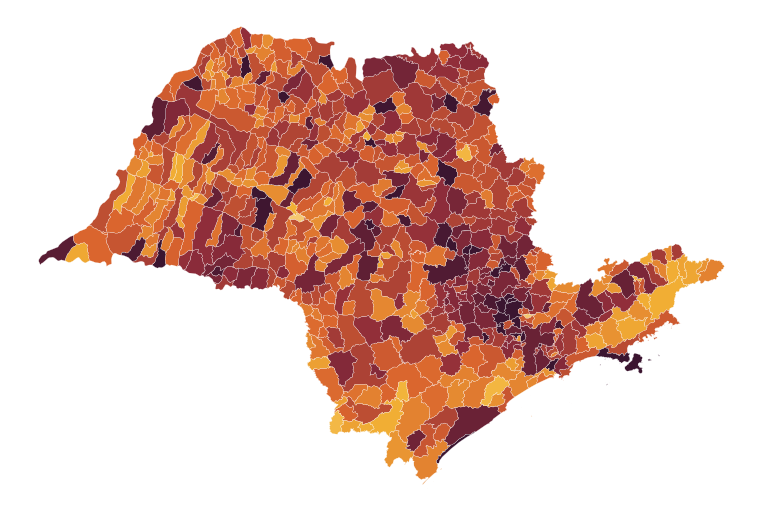
\includegraphics[width=\linewidth]{sp_official.png}
\column{0.32\textwidth}\centering
\eyebrow[cimg]{Predicted, never trained on SP}\\[2pt]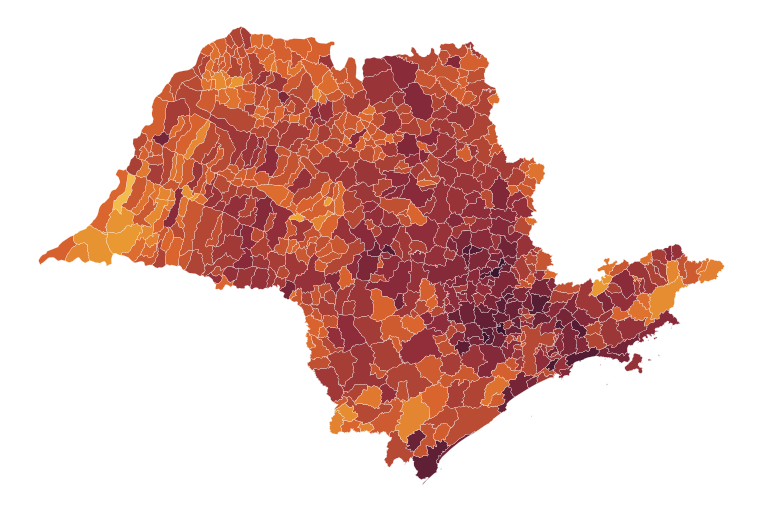
\includegraphics[width=\linewidth]{sp_predicted.png}\\[4pt]
\hspace*{-1.05\linewidth}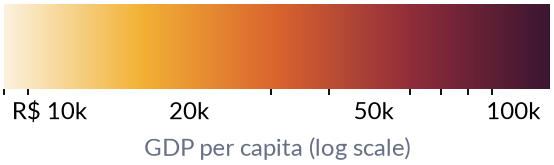
\includegraphics[width=0.95\linewidth]{cbar_gdp.png}
\column{0.32\textwidth}
\eyebrow{R\textsuperscript{2} against official GDP}\\[6pt]
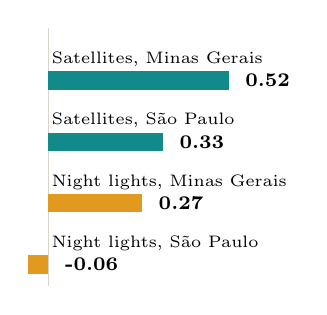
\begin{tikzpicture}[x=4.4cm,y=0.78cm]
  \draw[rule] (0,0.1) -- (0,-4.1);
  \foreach \v/\lab/\c [count=\i] in {0.52/{Satellites, Minas Gerais}/cimg,0.33/{Satellites, São Paulo}/cimg,
                                     0.27/{Night lights, Minas Gerais}/cntl,-0.06/{Night lights, São Paulo}/cntl} {
    \node[anchor=south west,font=\fontsize{6.5}{8}\selectfont,inner sep=1pt] at (0,-\i+0.42) {\lab};
    \fill[\c] (0,-\i+0.4) rectangle (\v,-\i+0.1);
    \node[anchor=west,font=\bfseries\fontsize{7.5}{9}\selectfont] at ({max(\v,0)+0.02},-\i+0.25) {\v};
  }
\end{tikzpicture}\\[4pt]
\fnote{\nSpMunis{} municipalities, models unchanged. Rank agreement \textbf{\nSpRho} (night lights \nSpNtlRho).
Minas Gerais 90\% range holds for \nSpRange; risk labels do not transfer.}
\end{columns}
\end{frame}

%======================== 15. THE APPLICATION ==========================
\begin{frame}{The application: GDP estimates where statistics are missing}
\begin{columns}[T,onlytextwidth]
\column{0.58\textwidth}
\framed{rule}{width=\linewidth}{app_guess.png}\\[3pt]
\fnote{Click a town: estimate, 90\% range and risk label; reveal the official value. Here: the iron-mine town, flagged high risk.}
\column{0.39\textwidth}
\eyebrow{What a user can do}\\[3pt]
\begin{enumerate}\setlength{\itemsep}{3pt}\fontsize{7.5}{9}\selectfont
  \item \textbf{Estimate any town} from satellite data, with an honest range and a warning when not to trust it.
  \item \textbf{Compare a new state}: São Paulo predicted vs official, by value or rank, against night lights.
  \item \textbf{See where satellites are blind}: risk groups and the largest misses, with reasons.
\end{enumerate}
\vspace{3pt}
\framed{rule}{width=0.72\linewidth}{app_transfer.png}\\[1pt]
\fnote{Works offline: \texttt{app/index.html}. Live demo now.}
\end{columns}
\end{frame}

%======================== 16. WHAT DID NOT WORK =======================
\setstage{7}
\begin{frame}{What did not work, and what it taught us}
\centering
{\renewcommand{\arraystretch}{1.5}\footnotesize
\begin{tabular}{@{}L{3.3cm}L{5.4cm}L{5.1cm}@{}}
\eyebrow{We tried} & \eyebrow{What happened} & \eyebrow[cntl]{Lesson}\\[-3pt]
\ing{cntl}{Night-light steering} & No gain once the aggregator was calibrated; an early ``steering helps'' result vanished & Calibration cut error \nCalibGain: fix the basics before adding ingredients\\
\ing{ctxt}{Text alignment} & Small gain, shrank in the rerun (\nRerunTextFrozen{} $\to$ \nRerunTextNew) & Frozen embeddings limit what text can add\\
\ing{cpoi}{POIs and roads} & Nothing on top of text & The fact sentences already carry them\\
\ing{cgdp}{Stage C vectors as an ``economic space''} & Similar-town search matches size, not wealth (R\textsuperscript{2} \nTwinPc); clusters explain \nClusterPc & The vectors work only inside the model; use estimates, not distances\\
\ing{muted}{Risk labels in a new state} & \nSpHighRisk{} São Paulo towns flagged high & Ranges travel; warnings need local recalibration\\
\end{tabular}}\par\vspace{6pt}
\fnote{All checks out-of-sample; details in the report and reports/tables (rerun\_check, stage\_c\_twins, clusters).}
\end{frame}

%======================== 17. ANSWERS AND LIMITS ======================
\begin{frame}{Answers to the five questions, and what we could not do}
\begin{columns}[T,onlytextwidth]
\column{0.53\textwidth}
\eyebrow{Research questions}\\[4pt]
{\renewcommand{\arraystretch}{1.32}\small
\begin{tabular}{@{}L{3.0cm}L{3.9cm}@{}}
RQ1 \ night-light steering & \chip{muted}{NO CLEAR EFFECT}\\
RQ2 \ text (captions) & \chip{ctxt}{SMALL GAIN, NOT ROBUST}\\
RQ3 \ POIs and roads & \chip{muted}{NOTHING ADDED}\\
RQ4 \ hybrid & \chip{cntl}{BEST, NOT SIGNIFICANT}\\
RQ5 \ where it fails & \chip{cgdp}{MINES, STEEL, COMMUTER TOWNS}\\
\textit{Beyond}: a new state & \chip{okc}{SATELLITES TRAVEL, LIGHTS DO NOT}\\
\end{tabular}}\\[6pt]
\fnote{Every answer out-of-sample on regions never seen; 95\% block-bootstrap intervals; confirmed by a full rerun.}
\column{0.43\textwidth}
\eyebrow{Limits}\\[3pt]
\begin{itemize}\setlength{\itemsep}{3pt}\footnotesize
  \item GSED is frozen: text can reorganise, not add, image information.
  \item Caption audit labelled by an LLM, one labeller, no agreement score yet.
  \item Stage C was revised after the first test results (choices made on validation).
  \item Trained on one state, transferred to one more; other countries and years untested.
  \item The tool cannot see mines or industry; it warns instead.
\end{itemize}
\end{columns}
\end{frame}

%======================== 18. CLOSING (night) ==========================
{\setbeamertemplate{background}{\nightbg}
\begin{frame}[plain]
\begin{tikzpicture}[remember picture,overlay]
  \node[anchor=east,inner sep=0,opacity=0.55] at ($(current page.east)+(0.3,0)$)
    {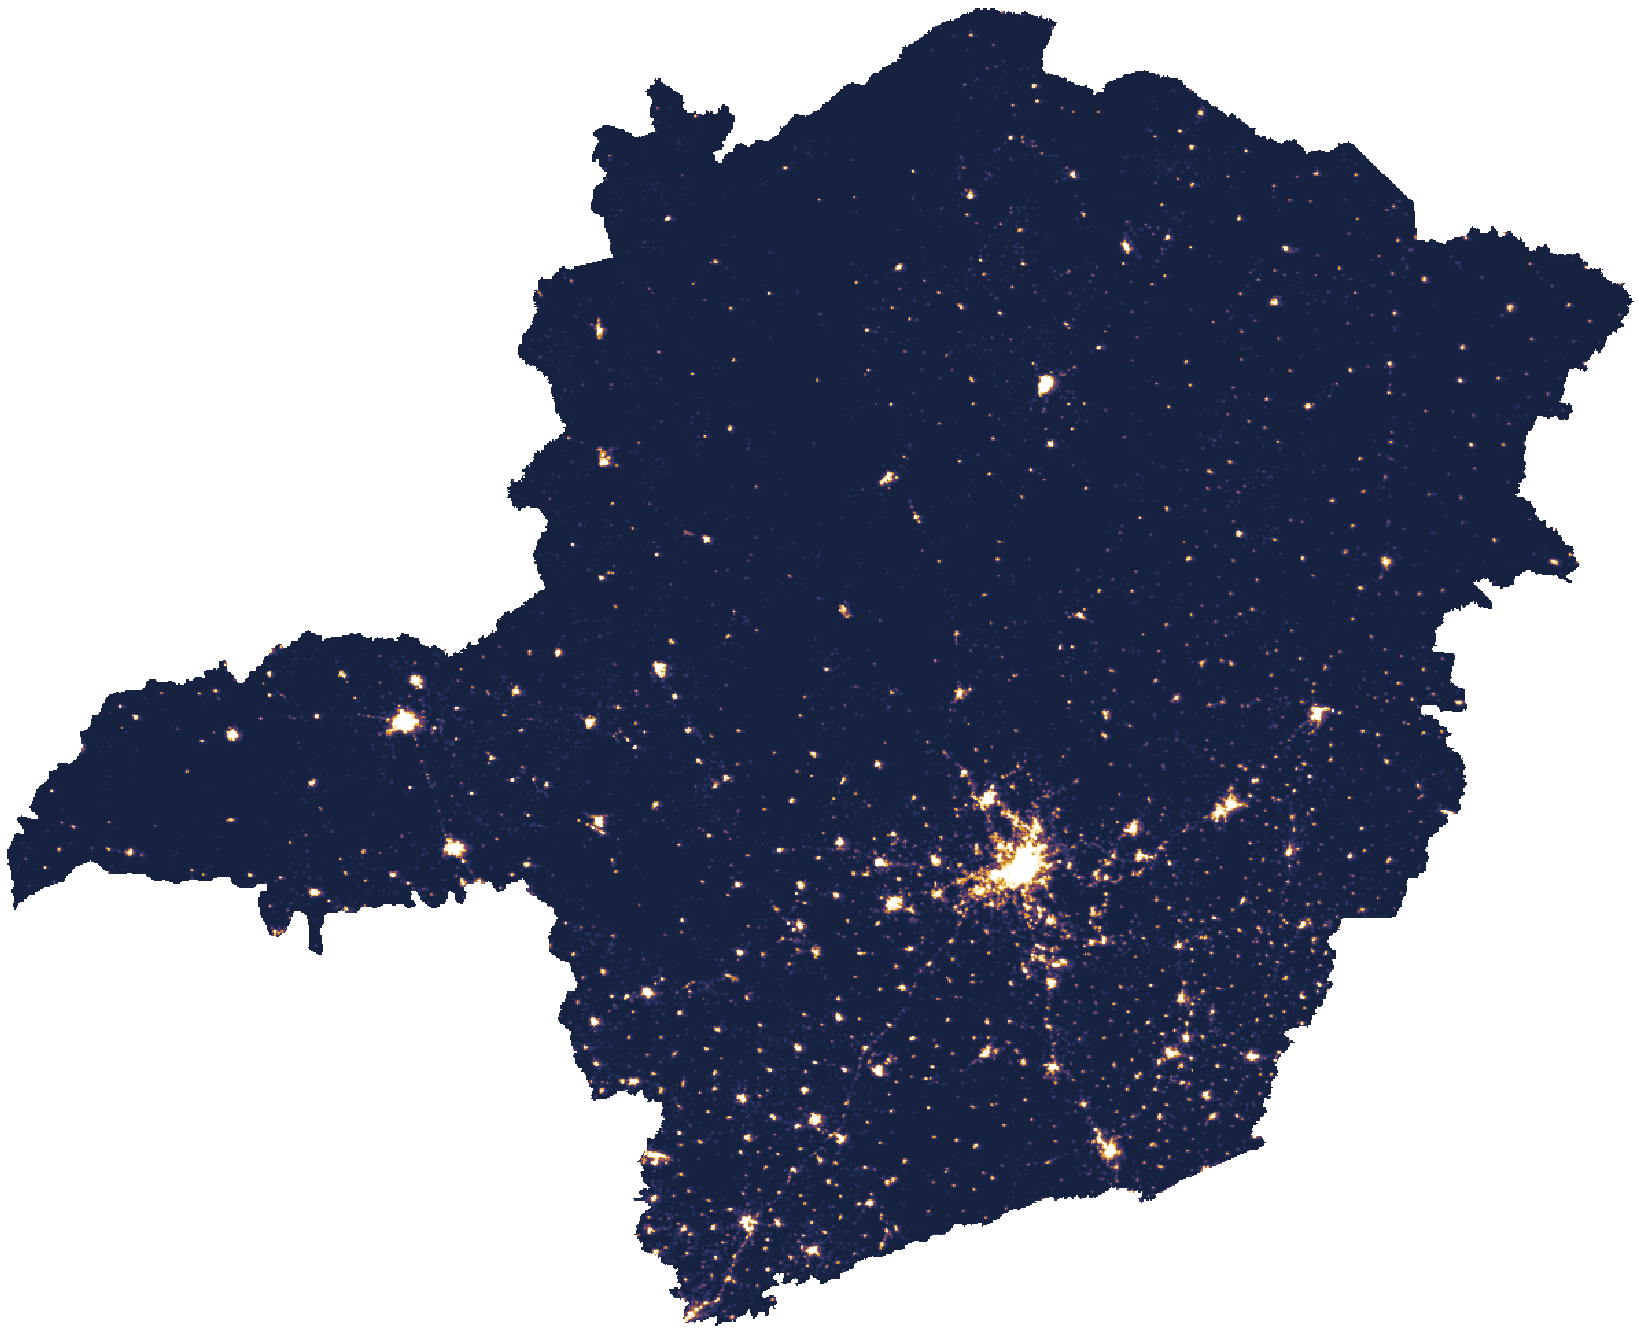
\includegraphics[height=0.9\paperheight]{hero_ntl.png}};
\end{tikzpicture}
\begin{minipage}{0.66\textwidth}\raggedright
\eyebrow[glow]{Take-away}\\[6pt]
{\blackfont\fontsize{15}{19}\selectfont\color{white}Free satellite data explain half of local income differences, keep working in a new state, and say when they cannot be trusted.\par}
\vspace{10pt}
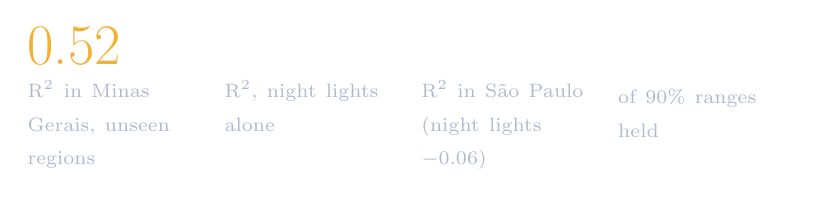
\begin{tikzpicture}[k/.style={anchor=north west,text width=2.3cm,align=left,inner sep=0}]
  \node[k] at (0,0) {{\blackfont\fontsize{22}{24}\selectfont\color{glow}\nHybridR}\\{\fontsize{7}{8.5}\selectfont\color{haze}R\textsuperscript{2} in Minas Gerais, unseen regions}};
  \node[k] at (2.5,0) {{\blackfont\fontsize{22}{24}\selectfont\color{white}\nNtlR}\\{\fontsize{7}{8.5}\selectfont\color{haze}R\textsuperscript{2}, night lights alone}};
  \node[k] at (5.0,0) {{\blackfont\fontsize{22}{24}\selectfont\color{white}\nSpR}\\{\fontsize{7}{8.5}\selectfont\color{haze}R\textsuperscript{2} in São Paulo (night lights \nSpNtlR)}};
  \node[k] at (7.5,0) {{\blackfont\fontsize{22}{24}\selectfont\color{white}\nCovNinety}\\{\fontsize{7}{8.5}\selectfont\color{haze}of 90\% ranges held}};
\end{tikzpicture}
\vspace{10pt}

{\footnotesize\color{haze}Steering, POIs and roads add nothing clear; text adds little.
\textbf{\color{white}Satellites miss what they cannot see:} mines, steel mills and commuter towns, and the tool warns about them.}\\[12pt]
{\blackfont\fontsize{16}{18}\selectfont\color{white}Questions?}\\[3pt]
{\fontsize{7.5}{9}\selectfont\color{haze}github.com/chadsaras/GIS\_Project \ $\cdot$ \ live demo: app/index.html}
\end{minipage}
\end{frame}}

%======================== B1. TEXT SPACE ===============================
\setstage{-1}
\begin{frame}{Backup: the text space speaks the state's economic geography}
\begin{columns}[c,onlytextwidth]
\column{0.4\textwidth}
\centering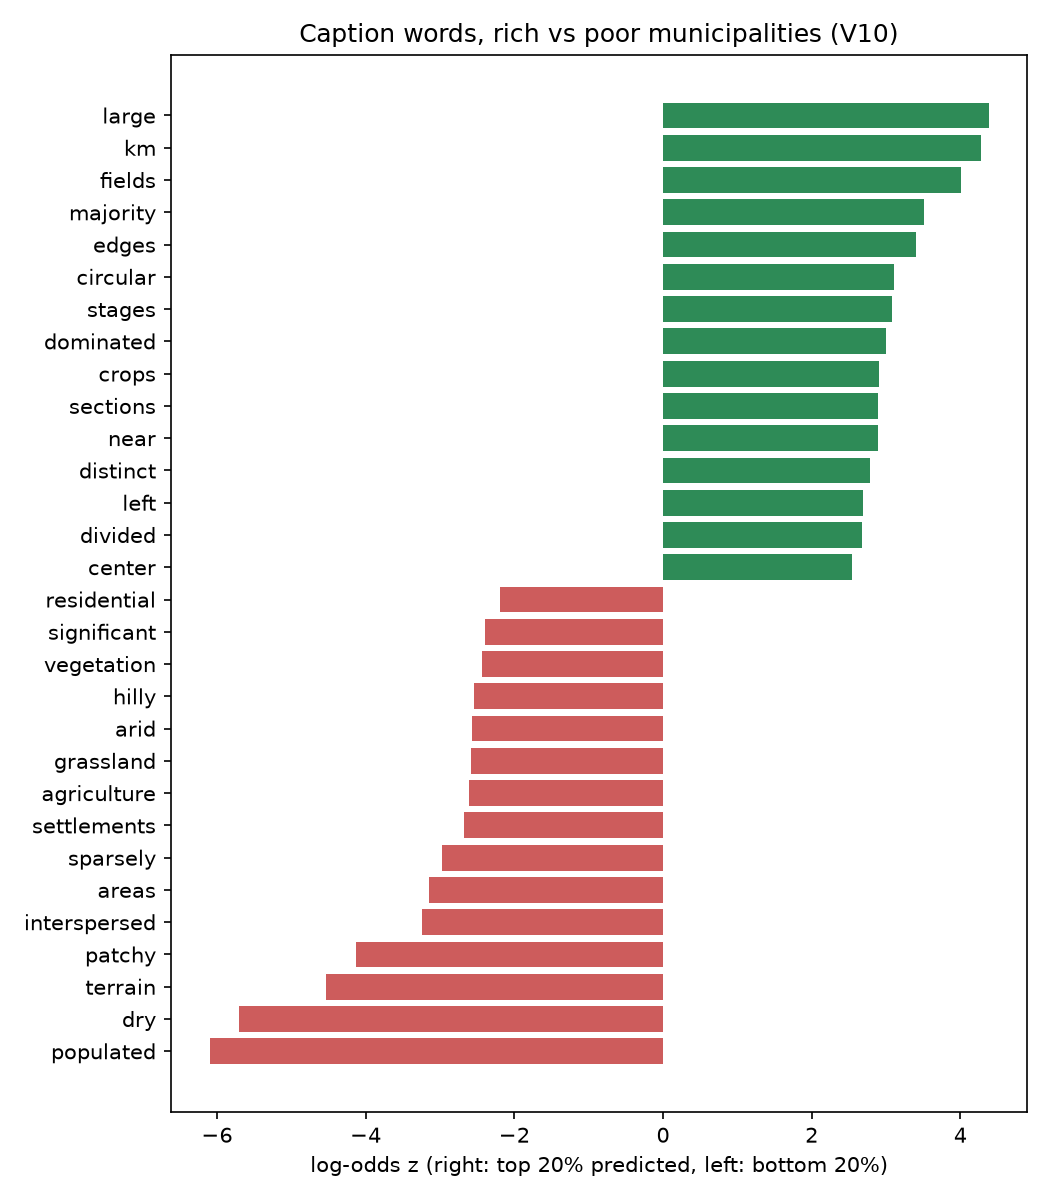
\includegraphics[height=5.6cm]{word_contrast.png}
\column{0.56\textwidth}
\eyebrow[okc]{Richest 20\% predicted}\\[1pt]
{\small \emph{large, fields, circular, crops, divided}: mechanised farming and centre pivots of the Triângulo}\\[8pt]
\eyebrow[cgdp]{Poorest 20\% predicted}\\[1pt]
{\small \emph{sparsely populated, dry, terrain, patchy, arid}: the semi-arid north and Jequitinhonha}\\[8pt]
\eyebrow[ctxt]{Nearest training captions}\\[2pt]
{\footnotesize \textbf{Belo Horizonte} (10.82 vs 10.91): dense grids of red-tiled roofs.\\
\textbf{Conceição do Mato Dentro} (11.94 vs 10.46): forest and pasture, so the mine stays invisible.}\\[6pt]
\fnote{Log-odds with informative Dirichlet prior (Monroe et al., 2008); official vs predicted log GDP per capita.}
\end{columns}
\end{frame}

%======================== B2. RERUN ====================================
\begin{frame}{Backup: a full rerun from scratch gives the same answers}
\begin{columns}[T,onlytextwidth]
\column{0.48\textwidth}
{\renewcommand{\arraystretch}{1.2}\footnotesize
\begin{tabular}{@{}lccc@{}}
\toprule
Model & R\textsuperscript{2} frozen & R\textsuperscript{2} rerun & $\Delta$RMSE\\
\midrule
V1 night lights & 0.271 & 0.271 & 0.000\\
V3 embeddings + C & 0.459 & 0.469 & $-$0.004\\
V4 + steering & 0.441 & 0.489 & $-$0.020\\
V6 + text + steering & 0.501 & 0.509 & $-$0.004\\
V7 full model & 0.502 & 0.519 & $-$0.007\\
\textbf{V10 hybrid} & \textbf{0.523} & \textbf{0.522} & 0.000\\
V12 LightGBM & 0.386 & 0.386 & 0.000\\
\bottomrule
\end{tabular}}
\column{0.48\textwidth}
{\renewcommand{\arraystretch}{1.3}\footnotesize
\begin{tabular}{@{}lcc@{}}
\toprule
Question & frozen & rerun\\
\midrule
RQ1 steering & +0.007 & $-$0.008\\
RQ2 text & $-$0.025 & $-$0.009\\
RQ3 POI, roads & $-$0.001 & $-$0.004\\
RQ4 hybrid & $-$0.009 & $-$0.002\\
\bottomrule
\end{tabular}}\\[6pt]
\fnote{$\Delta$RMSE of each comparison; every 95\% interval includes 0 in both runs, so every verdict is unchanged.
Deterministic steps match exactly; neural models differ by up to 0.02 RMSE (multi-threaded CPU training).}
\end{columns}
\end{frame}

%======================== B3. STAGE C VECTORS ==========================
\begin{frame}{Backup: Stage C vectors carry economy size, not wealth}
\begin{columns}[T,onlytextwidth]
\column{0.5\textwidth}
\eyebrow{Twins: 10 most similar training towns}\\[4pt]
{\renewcommand{\arraystretch}{1.25}\footnotesize
\begin{tabular}{@{}lcc@{}}
\toprule
Space & R\textsuperscript{2} income/person & R\textsuperscript{2} population\\
\midrule
Raw satellite vectors & 0.31 & 0.06\\
Population only & 0.00 & 0.99\\
Stage C, as trained & 0.22--0.33 & 0.74--0.81\\
Stage C, size removed & 0.28--0.41 & 0.19--0.47\\
\textit{The model itself} & \textit{0.46--0.52} & \\
\bottomrule
\end{tabular}}
\column{0.46\textwidth}
\eyebrow{Clusters: k-means, held-out towns}\\[4pt]
{\renewcommand{\arraystretch}{1.25}\footnotesize
\begin{tabular}{@{}lc@{}}
\toprule
Grouping by & R\textsuperscript{2} income/person\\
\midrule
Stage C vectors & 0.05--0.14\\
Land cover + lights & 0.17--0.23\\
Raw satellite vectors & 0.23--0.29\\
\bottomrule
\end{tabular}}\\[6pt]
\fnote{Stage C predicts total GDP and subtracts population at the end, so its vectors encode size. They are also
unstable across trained models (adjusted Rand 0.45 across rounds vs 0.90 for raw vectors).}
\end{columns}
\end{frame}

%======================== B4. CALIBRATION ==============================
\begin{frame}{Backup: calibration mattered more than night-light steering}
\begin{columns}[c,onlytextwidth]
\column{0.46\textwidth}
\centering\resizebox{\linewidth}{!}{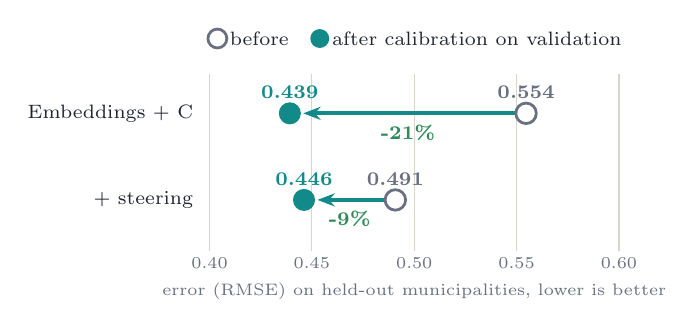
\begin{tikzpicture}[x=1cm,y=1cm,
  lab/.style={font=\fontsize{7.5}{9}\selectfont,text=ink,inner sep=0pt},
  num/.style={font=\bfseries\fontsize{7.5}{9}\selectfont,inner sep=1pt},
  tick/.style={font=\fontsize{6.5}{7.8}\selectfont,text=muted,inner sep=0pt}]
\draw[rule,line width=0.4pt] (0.00,0.5) -- (0.00,-1.75);
\node[tick,anchor=north] at (0.00,-1.83) {0.40};
\draw[rule,line width=0.4pt] (1.30,0.5) -- (1.30,-1.75);
\node[tick,anchor=north] at (1.30,-1.83) {0.45};
\draw[rule,line width=0.4pt] (2.60,0.5) -- (2.60,-1.75);
\node[tick,anchor=north] at (2.60,-1.83) {0.50};
\draw[rule,line width=0.4pt] (3.90,0.5) -- (3.90,-1.75);
\node[tick,anchor=north] at (3.90,-1.83) {0.55};
\draw[rule,line width=0.4pt] (5.20,0.5) -- (5.20,-1.75);
\node[tick,anchor=north] at (5.20,-1.83) {0.60};
\node[tick,anchor=north] at (2.60,-2.15) {error (RMSE) on held-out municipalities, lower is better};
\node[lab,anchor=east] at (-0.2,-0.00) {Embeddings + C};
\draw[-{Stealth[length=2.2mm]},cimg,line width=1.4pt] (3.88,-0.00) -- (1.19,-0.00);
\node[circle,draw=muted,fill=white,line width=1pt,minimum size=2.6mm,inner sep=0pt] at (4.02,-0.00) {};
\node[circle,fill=cimg,minimum size=2.8mm,inner sep=0pt] at (1.02,-0.00) {};
\node[num,text=muted,anchor=south] at (4.02,0.14) {0.554};
\node[num,text=cimg,anchor=south] at (1.02,0.14) {0.439};
\node[num,text=okc,anchor=north] at (2.52,-0.10) {-21\%};
\node[lab,anchor=east] at (-0.2,-1.10) {+ steering};
\draw[-{Stealth[length=2.2mm]},cimg,line width=1.4pt] (2.22,-1.10) -- (1.37,-1.10);
\node[circle,draw=muted,fill=white,line width=1pt,minimum size=2.6mm,inner sep=0pt] at (2.36,-1.10) {};
\node[circle,fill=cimg,minimum size=2.8mm,inner sep=0pt] at (1.20,-1.10) {};
\node[num,text=muted,anchor=south] at (2.36,-0.96) {0.491};
\node[num,text=cimg,anchor=south] at (1.20,-0.96) {0.446};
\node[num,text=okc,anchor=north] at (1.78,-1.20) {-9\%};
\node[circle,draw=muted,fill=white,line width=1pt,minimum size=2.4mm,inner sep=0pt] at (0.1,0.95) {};
\node[lab,anchor=west] at (0.25,0.95) {before};
\node[circle,fill=cimg,minimum size=2.4mm,inner sep=0pt] at (1.4,0.95) {};
\node[lab,anchor=west] at (1.55,0.95) {after calibration on validation};
\end{tikzpicture}
}
\column{0.5\textwidth}
\begin{enumerate}\setlength{\itemsep}{9pt}\small
  \item \textbf{Predictions were over-spread.} A straight-line correction fitted on validation municipalities
        cut error by {\bfseries\color{okc}\nCalibGain}.
  \item \textbf{Honest testing changes conclusions.} Steering looked helpful before the fix; after it, the gain vanished.
  \item \textbf{Disclosed:} the fix was chosen on validation data, but after the first test results were seen.
\end{enumerate}
\end{columns}
\end{frame}

\end{document}
